\begin{paper}{1}
\begin{header}
\title{On the theory of ferromagnetism}
\author{W. Heisenberg}
\location{Leipzig}
\note{Received on May 20th 1928.}
\makeheader
\end{header}

\begin{abstract}
The Weiss molecular force will be traced back to a quantum mechanical exchange phenomenon; and indeed it is like those exchange processes that have been proposed recently with success by Heitler and London for the meaning of the homopolar valence forces.
\end{abstract}

\section*{Introduction.} The ferromagnetic phenomena have been defined in a formally satisfactory manner by the well-known Weiss theory\footnote{\citeauthor{P. Weiss}, \citepub{Journ. de phys.} (e) \citevol{6}, \citepage{661}, \citeyear{1907} and \citepub{Phys. ZS.} \citevol{9}, \citepage{358}, \citeyear{1908}.}. This theory is based on the assumption that every atom in the crystal experiences a restoring force from the other atoms in the lattice which is to be proportional to the number of the \?{already restored}{bereits gerichteten} atoms. The origin of this atomic field was however completely unknown, and an explanation of the Weiss forces on the basis of the classical theory had the following obstacles: magnetic interaction forces between the atoms are always orders of magnitude smaller than the atomic fields following the ferromagnetic experiments. Electric interactions may lead to the correct order of magnitude; but one would expect that the electric interactions of two atoms would be proportional to the square of the cosine of their mutual angle of inclination rather than the cosine, contradicting the hypotheses of the Weiss theiry. Other difficulties were also discussed extensively by Lenz\footnote{W. Lenz, Phys. ZS. 21, 613, 1920.} and Ising\footnote{E. Ising, ZS. f. Phys. 31, 253, 1925.} has succeeded in also showing that the assumption of sufficiently great restoring forces between each two neighboring atoms in a chain is not sufficient to produce ferromagnetism.

In a new \?{study}{Stadium} the complex of questions surrounding ferromagnetism has been treated by the Uhlenbeck-Goudsmit theory of the spinning electron. Specifically, it follows from the well-known factor $g=2$ in the Einstein-de Haas effect (which indeed was just measured in ferromagnetic substances) that in a ferromagnetic crystal only the \?{magnetic moment}{magnetischen Eigenmomente} of the electrons, not the atoms, orient. Hence we again lose the possibility of interpreting the Weiss forces as electrical inreractions, independent of the relative spin-directions of the electrons, since we know that such forces do not exist. Further, Pauli\footnote{W. Pauli, ZS. f. Phys. 41, 81, 1927.} has been able to show that by neglecting the interaction of the electrons in a metal by applying the Pauli-Fermi-Dirac statistics, para- or diamagnetism always results.

\section{Foundations of the theory according to the model.} The basic idea of the theory proposed here is this: the empirical results place us with ferromagnetism in a very similar situation as we had found earlier with the results for the spectrum of the helium atom. It seemed at the time to follow from the \?{terms}{Termen} of the helium atom that a strong interaction energy reigned between the spin directions of the two electrons that led to a splitting of the \?{term system}{Termschemas} into the singlet and triplet systems. At the time this difficulty was solved by the \WTF{proof} that the apparently large interaction was indirectly brought about through a resonance or exchange phenomenon that is characteristic for all quantum mechanical systems of the same particles. So it is convenient to also invoke this exchange phenomenon for the explanation of the ferromagnetic phenomena.  We will attempt to show that the Coulomb interaction together with the Pauli principle is sufficient to cause the same effects as the molecular field postulated by Weiss. The mathematical methods for the treatment of such a complex problem have only been developed recently in the important investigations by Wigner\footnote{E. Wigner, ibid 40, 883, 1927; 43, 624, 1927.}, Hund\footnote{F. Hund. ibid 43, 788, 1927.}, Heitler and London\footnote{W. Heitler and F. London, ibid 44, 455, 1927, in the following cited as \ref{I}; W. Heitler, ibid, 46, 47, 1927 (cited as \ref{II}); ibid 47, 835, 1928 (cited as \ref{III}); F. London, ibid, 46, 455, 1928.}.

Before I get into the specific calculations, I would like to give a brief overview of the approximation methods that can be used in treating the motionof electrons in metals.

\begin{itemize}

\item
\textbf{Method I.} Following Pauli (loc cit) and Sommerfeld\footnote{A. Sommerfeld, ibid 47, 1, 1928; c.f. also W.V. Houston, ibid 47, 33, 1928 and C. Eckart, ibid 47, 38, 1928.}, the electrons will be supposed to be completely free to the first approximation. In the second approximation, some of the interactions with the lattice points will be addedas a perturbation (Houston\footnote{W.V. Houston. ZS. f. Phys. 48, 449, 1928.}). The interaction of the electrons among one another is completely ignored.

\item
\textbf{Method II.}
As a first approximation the motion of an electron in a periodic (in three directions) forcefield (which does not at all need to be small) will be calculated. In the next approximation some perturbations will be taken into account which arise from deviations from the periodicity in the lattice. The treatment of the interaction of the electrons among one another meets the same difficulty as with Method I.

\item
\textbf{Method III.}
In the first approximation one thinks of the lattice distance to be very large and assumes that each electron still belongs to its atom. In the next approximation one takes into account the exchange of electrons first treated by Heitler and London (loc cit\ref{I}), which moves, which move to different positions with the same energy in the unperturbed system. States in which are more electrons at an atom than in the unperturbed system will not be taken into account in this approximation.
\end{itemize}

The difference of these three systems becomes clearer if we explain them in another example, the Hydrogen molecule, which has been extensively treated by Heitler and London (loc cit\ref{I}). In method I the electrons would be treated as free, which naturally does not give not a suitable solution for calculating the molecule. In method II one would start from the solutions of the two-center problem (cf Hund\footnote{F. Hund, ibid 40, 742, 1927.}). In the limiting case of infinite distance from the nuclei electron 1 describes a $1 S$-orbit about nucleus $a$, electron 2 describes a $1 S$-orbit about nucleus $b$, a term would split into 4 terms (1 through 4) characterized by the table:

\begin{tabular}{c||c|c}
\hline\hline
 xyz & Nucleus $a$ & Nucleus $b$ \\
 \hline
 \hline
 1 & 1 & 2\\
 2 & 2 & 1\\
 3 & 1,2 & - \\
 4 & - & 1,2
\end{tabular}

The interaction of the two electrons would only be taken into account in higher approximations. -- Method III becomes directly identical with the method used by Heitler and London. Only term 1 and term 2 are \?{combined in}{zu...zusammengefa{\ss}t} an unperturbed system. Of term 3 and 4 it is assumed that they will lead to markedly higher energy values. The term manifold of the unperturbed system is therefore \?{lower}{geringer} than in Methods I and II.

There is probably no a priori argument for preferring any one of the three approximation procedures over the others. Method I will be most applicable with metals with very large \?{conductance}{Leitfahigkeit}, Method III with metals with smaller conductance. Method II stands in the middle between these two limiting cases.

For the following calculations I have used Method III, since only it permits a quantitative treatment of the electron interaction.

\section{The distribution of term values.} The following calculations form a simple generalization of Heitler-London's investigation (loc cit\ref{I}) to the cast of $2n$ interacting electrons (the number of electrons is assumed to be even on purely formal grounds). So in the unperturbed system there are $2n$ electrons found in $2n$ different quantum cells (while not differing in energy, probably differing in position).

About the electrons' quantum numbers in their atoms we initially only make the assumption that they are equal for all atoms. Other stationary states of the unperturbed system will not be taken into account, it is assumed that they would lead to much higher energy values.

Then the task is the determination of the energy values of the stationary states of the whole system which are associated with the above-described state, if it is considered as a perturbation of the Coulomb interaction of the changes of one atom with the charges of any other atom. Because of the great computational complications that would occur otherwise, it will only be possible for us to pursue the perturbation calculation up to the first approximation. Whether this first approximation is really sufficient for the cases that occur in nature remains to be seen. For the eigenfunctions of the unperturbed system we take products of the Schr\"odinger eigenfunctions of the hydrogen atom, or better those eigenfunctions corresponding to the relevant \WTF{Atomrest}, just as in the cited article by Heitler and London; — it is probably superfluous to repeat those ideas hear in detail. Though these eigenfunctions are not orthogonal, the deviation from the usual treatment that would be required here is apparent only in terms of the second order, so we can consistently apply the usual manner of treatment in the case of orthogonal eigenfunctions. As a consequence of the mutual perturbation, the electrons of an atom can act with those of any other by exchange. As long as the perturbation terms of second order are ignored, there are only simple transpositions between two neighboring atoms. Assuming, as the simplest case, that in the unperturbed system each atom had one valence electron, then the "exchange terms" of the perturbation energy are reduced to the expressions given by Heitler and London
\uequ{
J_{(kl)} = \frac{1}{2}\int\psi_k^\chi \psi_k^\lambda \psi_l^\chi \psi_l^\lambda \left(
\frac{2e^2}{r_{kl}} + \frac{2e^2}{r_{\chi\lambda}} - \frac{e^2}{r_{\chi k}} - \frac{e^2}{r_{\chi l}} - \frac{e^2}{r_{\lambda k}} - \frac{e^2}{r_{\lambda l}}
\right)\D{\tau_k}\D{\tau_l}
}
Here $k$ and $l$ denote the labels of two electrons, $\chi$ and $\lambda$ denote the labels of the \?{atoms}{Atomreste} to which $k$ and $l$ belonged in the unperturbed system.  As a further important constant, the pure "static" interaction enters into the perturbation calculation:
\uequ{
J_E = \int\D{\tau_1}\d\tau_2\dots\d\tau_{2n}(\psi_1^1)^2(\psi_2^2)^2\dots(\psi_{2n}^{2n})^2\\
\left\{
\sum\limits_{k < l}\frac{e^2}{r_{kl}} +
\sum\limits_{\chi > \lambda}\frac{e^2}{r_{\chi\lambda}} -
\sum\limits_{k \neq \lambda}\frac{e^2}{r_{k\lambda}}
\right\}.
}

The magnetic interactions are left completely out of consideration because of their smallness. Nevertheless by virtue of the exchange processes the spin moments of all the electrons will be partly parallel, partly anti-parallel. If we add Pauli's fundamental assumption that the eigenfunctions of the total system are to be antisymmetric in each electron, then to each term value of the perturbed system there is a totally definite total magnetic moment characterized by the angular momentum $s\frac{h}{2\pi}$. In total there are (ignoring the Pauli principle and spin) $(2n)!$ terms in the perturbed system. A statistical treatment of ferromagnetism becomes possible if each energy values are calculated that belong to a given value of $s$. This task is however not solvable in this form, since $2n$ is a large number. We could only hope to get a general view of the distribution of the eigenvalues at a given $s$. In the following we will work out the number of terms, the \WTF{Energieschwerpunkt} so the mean value of the energy with a given $s$ and the mean square fluctuation of the energy at this mean value. Then if we make the somewhat arbitrary assumption that the energy values in the first approximation are distributed in a Gaussian error curve about the mean value where the breadth of the error curve is calculated from the square fluctuation.

Following the investigations by Wigner, Hund and Heitler (loc cit),  y the assumption of the Pauli principle each value $s$ of the total spin moment is associated with a term system ("$\sigma$") characterized by a certain partition of $2n$ into summands:
\nequ{3}{
2n = \underbrace{2 + 2 + \dots + 2}_{(n-s)\text{-times}} + \underbrace{1+\dots+1}_{2s\text{-times}}
}

The partition of the "reciprocal" system is then
\nequ{4}{
2n = (n - s) + (n + s).
}

Heitler (loc cit\ref{II}) has given the formula for the mean value of the energy in the system $\sigma$, the \WTF{Energieschwerpunkt}:
\nequ{5}{
E_\sigma = \frac{1}{f_\sigma}\sum\limits_P \chi_\sigma^P J_P.
}

Here $\chi_\sigma^P$ denotes the group character associated with the permutation $P$, $f_\sigma = \chi_\sigma^E$ is the number of terms in the system. The energy of the unperturbed system is left out as an additive constant. — We further calculate the mean value of the squared fluctuation $\overline{\Delta E^2}$ of the about the value $E_\sigma$: the energy values are found as the root of a $f_\sigma$-order equation obtained by setting the determinant
\nequ{6}{
\left|
\begin{array}{lll}
\sum\limits_P b_{11}^P J_P - x &
\sum\limits_P b_{12}^P J_P \dots &
\sum\limits_P b_{1f}^P J_P \\
\sum\limits_P b_{21}^P J_P &
\sum\limits_P b_{22}^P J_P - x\dots &
\vdots \\
\vdots & \, & \vdots \\
\sum\limits_P b_{f1}^P J_P & \dots & 
\sum\limits_P b_{ff}^P J_P - x
\end{array}
\right| = 0
}
equal to zero. The sum of the roots of this equation $\sum x_n$ is given by the coefficients of $x^{f-1}$, so $\sum\limits_{i,P}b_{ii}^P J_P = \sum\limits_P \chi_\sigma^P J_P$, which leads to equation (5). The sum $\sum\limits_{n>m} x_n x_m$ is given by the coefficients of $x^{f-2}$ in (6), and hence
\nequ{7}{
\sum\limits_{n>m} x_n x_m &= 
\sum\limits_{i>k}\sum\limits_{P,P'} b_{ii}^P b_{kk}^{P'} J_P J_{P'} - 
\sum\limits_{i>k}\sum\limits_{P,P'} b_{ik}^P b_{ki}^{P'} J_P J_{P'}\\
&= \frac{1}{2}\left(
\sum\limits_{i,k}\sum\limits_{P,P'} b_{ii}^P b_{kk}^{P'} J_P J_{P'} -
\sum\limits_{i,k}\sum\limits_{P,P'} b_{ik}^P b_{ki}^{P'} J_P J_{P'}
\right).
}
In the last expression $i, k$ is independently summed over all values. Now $\sum\limits_k b_{ik}^P b_{ki}^{P'}$ denotes the $\Nth{i}$ diagonal term of the product matrix $b^P\cdot b^{P'}$. Since the matrices $b$ form a representation of the group,
\uequ{
b^P\cdot b^{P'} = b^{P\cdot P'}.
}
Observing that $\chi^P = \sum\limits_i b_{ii}^P$ it follows that
\nequ{8}{
\sum\limits_{n>m}x_n x_m = \frac{1}{2}\sum\limits_{PP'}\left(
\chi^P\chi^{P'} - \chi^{P\cdot P'}\right)J_P J_{P'}.
}

If we set $x_n = E_\sigma + \Delta E_n$ (the index $\sigma$ here is actually associated with $x_n, \Delta E_n$ as well; we leave it out for clearer notation), then
\nequ{9}{
\sum\limits_{n>m} x_n x_m &= \sum\limits_{n>m}(E_\sigma + \Delta E_n)(E_\sigma + \Delta E_m) \quad \text{($n,m=1,\dots,f_\sigma$)}\\
&= \frac{f_\sigma(f_\sigma - 1)}{2}E_\sigma^2 + 
\sum\limits_{n>m}\Delta E_n \Delta E_m;
}
because $\sum\Delta E_n = 0$,
\nequ{10}{
\sum\limits_{n=1}^{f_\sigma}\Delta E_n^2 =
 -2\sum\limits_{n>m}\Delta E_n \Delta E_m.
}

From (5), (8), (9), (10) and the equation $f_\sigma = \chi_\sigma^E$ it finally follows that
\nequ{11}{
\sum\limits_{n=1}^{f_\sigma}\Delta E_n^2 = \frac{1}{f_\sigma}
\sum\limits_{PP'}(\chi_\sigma^E \chi_\sigma^{P\cdot P'} - 
\chi_\sigma^P \chi_\sigma^{P'})J_P J_{P'}
}
and
\nequ{12}{
\overline{\Delta E_\sigma^2} = \frac{1}{f_\sigma^2}\sum\limits_{PP'} (\chi_\sigma^E \chi_\sigma^{P\cdot P'} - 
\chi_\sigma^P \chi_\sigma^{P'})J_P J_{P'}.
}

To be able to apply these formulae, we would still have to work out the group character for the permutations of the various classes. Since all the $J_P$ vanish with the exception of the cases $P=E$ and $P$ of the class of (12) (transpositions), for $\chi_\sigma^{P\cdot P'}$ only the following types come into consideration:
\uequ{
\chi_\sigma^E, \chi_\sigma^{(1\,2)}, \chi_\sigma^{(1\,2\,3)}, \chi_\sigma^{(1\,2)\,(3\,4)}
}

This group character could be calculated following a method of Schur described by Heitler (loc cit\ref{III}). It immediately gives for the reciprocal term system\footnote{The values given by Heitler (loc cit \ref{III}, equation (32)) for $f_\sigma$ and $\chi_\sigma^{(1\,2)}$ were obscured by printing errors.}:
\nequ{13}{
\chi_{n-s,n+s}^E &= \frac{(2n)!(2s+1)}{(n-s)!(n+s+1)!},\\
\chi_{n-s,n+s}^{1\,2} &= \frac{(2n-2)!2(2s   +1)}{(n-s)!(n+s+1)!}
(s^2 + s + n^2 - 2n),\\
\chi_{n-s,n+s}^{1\,2\,3} &= \frac{(2n-3)!2(n-1)}{(n-s)!(n+s+1)!}
\left\{6s^2 + 9s^2 + s(2n^2 - 10n + 3) + n(n-5)\right\},\\
\chi_{n-s,n+s}^{(1\,2)(3\,4)} &= \frac{4(2n-4)!}{(n-s)!(n+s+1)!}\left\{
2s^5 + 5s^4 + 4s^3(n^2 - 5n + 4) \right.\\
&\quad\quad\quad\quad \quad\quad\quad\quad \quad\quad\quad\quad + s^2(6n^2 - 6n^3 + 15n^2 \\
&\quad\quad\quad\quad \quad\quad\quad\quad \quad\quad\quad\quad - 14n + 3) + n^4 - 6n^3 \\
&\quad\quad\quad\quad \quad\quad\quad\quad \quad\quad\quad\quad\left. + 14n^2 - 9n\right\}
}

The character of the actually-occurring term systems are distinguished from the character of their reciprocals only by the sign. And indeed the character of the reciprocal system is equal resp. equal and opposite of the system itself when the permutation $P$ arises from an even resp. odd number of transpositions.

Up to now, everything has applied in complete generality, without reference to the specific assumptions that we have made about the crystal lattice or the \WTF{Atombau der ferromagnetischen Substanz}.

We must now further specialize our assumptions to be able to calculate.  It immediately follows from (1) and Heitler and London's calculations that $J_{(12)}$ exponentially decreases with increasing distance. An atom in a lattice with thus in the main only enter into exchanges with its "neighbors"; the exchange with any atom that is further than the "neighboring atoms" will on the other hand be negligible. The number of "neighbors" of an atom is e.g. 1 in a molecular lattice of diatomic molecules, 2 in a linear chain, 4 in a \?{plane square lattice}{quadratischen Fl\"achengitter}, 6 in a simple cubic lattice, 8 in a cubic body-centric lattice, 12 in a cubic face-centric lattice.

We further make the assumption that all non-vanishing exchange terms $J_P$ should be equal (we call this value $J_0$). This must be the case if the \WTF{Atomreste} are unmagnetic, i.e. centrally-symmetric. So we now calculate $E_\sigma$, $\overline{\Delta E_\sigma^2}$ for a lattice in which each atom has $z$ neighbors. Only the highest powers of $n$ and $s$ will be taken into account and lower terms are omitted; this means that we ignore the effects at the boundary surfaces.

The number of transpositions that lead to the value $J_0$ (i.e. the number of pairs of atoms of smallest distance) is $\frac{x\cdot 2n}{2} = z\cdot n$. So from (5) and (13) it follows that
\nequ{14}{
E_\sigma = -z\cdot\frac{s^2+n^2}{2n}J_0 + J_E.
}

For calculating the value of $\overline{\Delta E_\sigma^2}$ we first need the value of the expression
\nequ{15}{
A_{P,P'} = \frac{1}{f_\sigma^2}
\left(\chi^E\chi^{P\cdot P'} - \chi^P\chi^{P'}\right)
}
for the various possible combinations of $P$ and $P'$. It gives (up to smaller powers of $n$ and $s$):
\begin{enumerate}
	\item $P=P'$
	\nequ{16.1}{
	A_{(12)(12)} = \frac{(n^2-s^2)(3n^2+s^2)}{4n^4}
	}
	\item $P$ and $P'$ have one element in common
	\nequ{16.2}{
	A_{(12)(13)} = \frac{(n^2-s^2)s^2}{4n^4}
	}
	\item $P$ and $P'$ have no elements in common
	\nequ{16.3}{
	A_{(12)(34)} = \frac{-(n^2-s^2)s^2}{2n^5}
	}
\end{enumerate}

If an atom has $z$ neighbors, then type 1 occurs $z\cdot n$ times, type 2 $z(z-1)n$ times, type 3 $\frac{z^2 n^2}{2}$ times.

Finally, according to equation (12),
\uequ{
\overline{\Delta E_\sigma^2}=J_0^2=\left(
zn\cdot A_{(12)(12)} + 2z(z-1)n A_{(12)(13)} + 2\frac{z^2 n^2}{2}A_{(12)(34)}
\right)
}
and
\nequ{17}{
\overline{\Delta_\sigma^2}  = J_0^2 z \frac{(n^2-s^2)(3n^2-s^2)}{4n^3}.
}

The mean deviation of the energy from the mean value (14) is thus of order $\Delta_\sigma \approx J_0 \sqrt{n}$. -- $\sigma$ always denotes in the previous formulae the term system associated with the partition (3) and hence total spin $s$.

\section{Statistics; connection to the Weiss formulae.}

For the following considerations, the above-mentioned, though somewhat arbitrary assumption that the distribution of the energy values about the mean has approximately the form of a Gaussian error curve. Since the total number of the terms associated with the spin $s$ is $f_\sigma$\footnote{Without the Pauli principle, because of the $f_\sigma$-fold degeneracy, the total number of terms in all systems associated with the partition would be equal to $f_\sigma^2$. But, the degeneracy will be ruled out by the pauli principle.}, we assume that
\uequ{
\frac{f_\sigma}{\sqrt{2\pi \overline{\Delta E_\sigma^2}}}\cdot
\exp{-\frac{\Delta E^2}{2\overline{\Delta E_\sigma^2}}} d\Delta E\text{ terms}
}
lies between $E_\sigma + \Delta E$ and $E_\sigma + \Delta E + d\Delta E$.

After the previous calculations the direction of the total spin $s$ in the crystal remains totally undetermined if, as we might conclude from the results of the Einstein-de Haas effect, the \?{orbital angular momentum}{Bahnmomente} of the electrons in the crystal is compensated. If we now place the crystal in an external magnetic field of strength $H$, then there arises in addition to the internal energy which depends on $s$ an external energy which depends on the projection $m$ of $s$ on the external field. According to the well-formulae, for this additional energy ($g=2$ for the spin!)
\nequ{18}{
E' = -\frac{e}{\mu c}\frac{h}{2\pi}H\cdot m \text{ ($s\geq m \geq -s$)}
}
($\mu$ = electron mass).

Now the task is, for a given temperature and a given value of $H$, to work out the most likely value of $m$. We introduce the abbreviations
\nequ{19}{
\alpha &= \frac{1}{kT}\cdot\frac{e}{\mu c}H\cdot\frac{h}{2\pi},\\
\beta &= \frac{z J_0}{kT}.
}

Then, one forms the \?{sum over states}{Zustandssumme} (up to an innessential factor that is independent of $\alpha$):
\uequ{
\sum\limits_{s=0}^n\sum\limits_{m=-s}^{+s}\int\limits_{-\infty}^{+\infty}
\d\Delta E & \frac{f_\sigma}{\sqrt{2\pi\overline{\Delta E_\sigma^2}}}\cdot
\exp{\alpha m + \beta\frac{s^2}{2n} - \frac{\Delta E}{kT} - \frac{\Delta E^2}{2\overline{\Delta E_\sigma^2}}}\\
& = \sum\limits_{s=0}^n\sum\limits_{m=-s}^{+s}f_\sigma
\exp{\alpha m + \beta \frac{s^2}{2n} + \frac{\overline{\Delta E_\sigma^2}}{2k^2 T^2}}.
}
Finally, from (17) (again ignoring unimportant factors),
\nequ{20}{
S= \sum\limits_{s=0}^n\sum\limits_{m=-s}^{+s}
f_\sigma \exp{\alpha m + \beta\frac{s^2}{2n} - \beta^2\frac{s^2(4n^2-s^2)}{8n^3z}}
}
Denoting the expression $\exp{\beta\frac{s^2}{2n} - \beta^2\frac{s^2(4n^2-s^2)}{8n^3z}}$ by $g(s)$ and reflecting that $f_\sigma = \binom{2n}{n+s}$, and after reversing the order of summation:
\uequ{
S=\sum\limits_{m=-n}^{+n}\sum\limits_{s=|m|}^n\exp{\alpha m}\cdot
g(s)\left[\binom{2n}{n+s} - \binom{2n}{n+s+1}\right],
}
and by a rearrangement analogous to partial integration:
\uequ{
S&=S_1+S_2 = \sum\limits_{m=-n}^{+n}\exp{\alpha m}g(m)\binom{2n}{m+m}\\
& + \sum\limits_{s=0}^{n}\sum\limits_{m=-s}^{+s}\exp{\alpha m}\left(
g(s+1)-g(s)\right)\binom{2n}{n+s+1},\\
S_2 &= \sum\limits_{s=0}^n\frac{\exp{\alpha(s+1)} - \exp{-\alpha s}}{\exp\alpha - 1}\cdot\left(g(s+1)-g(s)\right)
\binom{2n}{n+s+1}.
}
Since $g(s)$ is an even function of $s$, in the approximation used throughout, the term with $\exp{-\alpha s}$ can be removed from $S_2$ and the sum for it taken from $s=-n$ to $s=+n$. It is then seen that, up to factors of order 1, $S_2$ also takes the form of $S_1$ (if the summation index $s$ in $S_2$ are replaced by $m$).

Finally, it follows that
\nequ{21}{
S=F\cdot\sum\limits_{-n}^{+n}\exp{\alpha m}g(m)\binom{2n}{m+n},
}
where $F$ is a function of the quantities $\alpha$ and $\beta$ of order 1 (when $\alpha$ and $\beta$ are of this order).

For further calculation it is assumed that the $S$ under the summation symbol exhibits a steep maximum at the point $m=m_0$ ($m_0 \approx$ the mean value of $m$), which shall be verified later. We set $m=m_0 + (m-m_0)$ and, in the exponent of $g(m)$, expand in powers of $(m-m_0)$. It yields:
\uequ{
g(m) \approx \exp{\beta \frac{m_0^2}{2n} + \beta\frac{m_0}{n}(m-m_0) - \frac{\beta^2}{8n^3 z}\left[4m_0^2 n^2 - m_0^4 + 8m_0n^2(m-m_0)-4m_0^3(m-m_0)\right]}.
}
So $S$ becomes, again up to an inessential factor that does not depend on $\alpha$,
\nequ{22a}{
S&=F\sum\limits_{m=-n}^{m=n}\exp{\left(
\alpha + \beta\frac{m_0}{n} - \beta^2\frac{m_0}{nz} + \beta^2\frac{m_0^3}{2n^3z}
\right)m} \binom{2n}{m+n}\\
&= F\left[2\mathfrak{Cos}\left(
\frac{\alpha+\beta\frac{m_0}{n}-\beta^2\frac{m_0}{nz} + \beta^2\frac{m_0^3}{2n^3z}}{2}
\right)\right]^{2n}.
}
From $S$ we obtain the most probable value $w_0$ in the well-known manner, according to the equation
\nequ{22}{
m_0=\pX{}\pY{\alpha}\log{S} = n \mathfrak{Tg} \frac{\alpha+\beta\frac{m_0}{n}-\beta^2\frac{m_0}{nz} + \beta^2\frac{m_0^3}{2n^3z}}{2}.
}
The part arising from the differentiation of $\log{F}$ is negligible against $n$. Therein also lies the belated justification for only taking into account the highest powers in $n$ and $s$, and hence ignoring factors of order 1.

Formula (22) is essentially identical to the well-known Weiss formula for Ferromagnetism. That in (22) $\mathfrak{Tg}x$ takes the place of $\mathfrak{Cotg}x-1/x$ (as in Weiss) arises from the fact that for a spin moment, only two positions are possible in an external field. If one puts
\nequ{23}{
\frac{m_0}{n} = y\text{; }
\alpha+\beta\frac{m_0}{n}-\beta^2\frac{m_0}{nz} + \beta^2\frac{m_0^3}{2n^3z} = 2x,
}
then the following equations hold:
\nequ{24.I}{
y=\mathfrak{Tg}x,
}
\nequ{24.II}{
2x = \alpha + y(\beta - \frac{\beta^2}{x}) + \frac{\beta^2}{2z}y^3.
}
These formulae are distinguished from Weiss's formulae by the cubic part in (24.II). The solutions of (24) are again most easily constructed graphically. Figure 1 is drawn with the values $\alpha=0.2; \beta=2; z=8$.
\begin{figure}[h]
	\begin{center}
		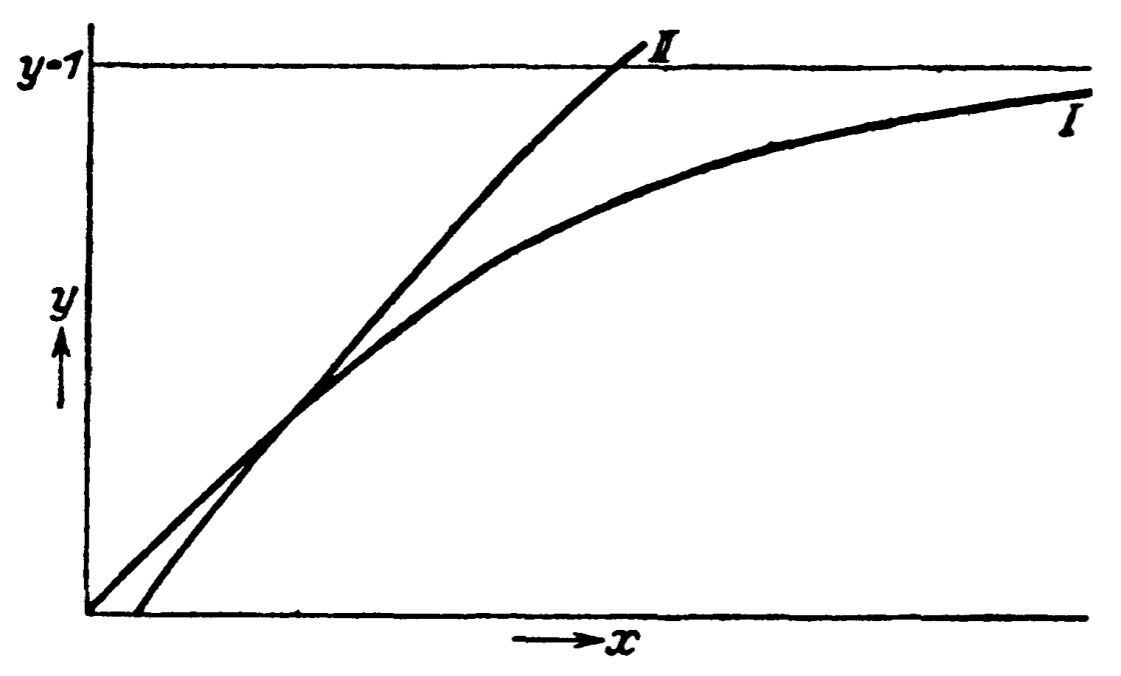
\includegraphics[width=150pt]{fig1}
	\end{center}
\end{figure}

Small or negative values of the constant $\beta$ provide paramagnetism. Ferromagnetism happens when the tangent of curve II for $y=0$ makes a smaller angle with the $x$-axis than the tangent of I; here the influence of the cubic part is ignored. The condition for ferromagnetism then reads
\nequ{25}{
\beta\left(1-\frac{\beta}{z}\right)\geq 2.
}
This condition can only be met for high values of $z$. The maximal value of the left side of (25) is $\left(\beta_\text{max} = \frac{z}{2}\right)\frac{z}{2}\left(1-\frac{1}{2}\right)$, and it follows that:
\nequ{26}{
z\geq 8.
}

Accordingly, ferromagnetism is only possible for the types of lattices in which an atom has at least eight neighbors. For $\El{Fe}$, \El{Co}, \El{Ni} this is the case, the lattices are all cubic, some body-centric ($z=8$), some face-centric ($z=12$). -- Taking into consideration the third degree part in (24.II) it can happen for $z=7$ that though curve II (for $\alpha=0$) increases more quickly than I at the zero point, further up there are still two intersections between I and II. But since $n=7$ never occurs, no physical significance will be attached to this possibility.

If $\beta$ increases over the value $z/2$ (increasing $\beta$ corresponds with decreasing temperature), then the "strength of the molecular field" again decreases according to equation (25), for $\beta > \frac{z}{2}\left(1+\sqrt{1-\frac{8}{z}}\right)$ there is only paramagnetism. We do not believe that this result has any physical significance. Mathematically it comes to pass that because of the assumed Gaussian distribution of the energy values, which has as a consequence that even for small values of $s$ there are term values that (for positive $J_0$) lie just as low or lower than the energy, associated with $s=n$. The deviations of the actual energy distribution curves from the assumed values are naturally made more and more apparent at decreasing temperatures.

Thus the provisional theory attempted here must be improved by working out the higher mean fluctuation values $\overline{\Delta E^2}$, $\overline{\Delta E^4}$ etc and constructing accordingly improved distribution curves for the term values. In this improved theory there will be corresponding higher powers of $\beta$ on the left side of (25); the left side of (25) is actually a transcendental function of $\beta$; the value for the left side of (25) that we have found here will correspond to an expansion of this function in powers of $\frac{\beta}{z}=\frac{J_0}{kT}$ truncated at the second term (our $\beta-\frac{\beta^2}{z}$ could probably only differ by a small part from the first two terms of the true power series of that function). From these reflections however it follows that for higher values of $\frac{\beta}{z}$, say $\frac{\beta}{z}\gtrsim\frac{1}{2}$, an investigation of higher order fluctuations $\overline{\Delta E^n}$ is indispensable for the study of ferromagnetism. Such a closer investigation of the distribution curve will also probably shift the boundary value of $z$. But it will probably not qualitatively change our results much. 

If $\beta$ is markedly smaller than the boundary value given by (25), then equation (24) gives paramagnetism, as already mentioned. For small values of $\alpha$ ($\mathfrak{Tg} x \approx x - \frac{x^3}{3}\dots$) the calculation gives:
\nequ{27}{
y=\frac{\alpha}{2-\beta+\frac{\beta^2}{z}} + 
\frac{\alpha^3}{\left(2-\beta+\frac{\beta^2}{z}\right)^4}\left(
\frac{\beta^2}{2z} - \frac{2}{3}\right) + \dots.
}
The first term of this series gives the Curie law with one modification, similar as in the Weiss theory:
\uequ{
m_0\,\,\text{prop}\frac{1}{T-\Theta}\frac{T}{T\left(1+\sqrt{1-\frac{8}{x}}\right) - \Theta\left(1-\sqrt{1-\frac{8}{x}}\right)}.
}
Here the critical temperature is
\uequ{
\Theta=\frac{2J_0}{k\left(1-\sqrt{1-\frac{8}{x}}\right)}.
}

Before turning to the discussion of the numerical value of $J_0$, I will justify the claim made earlier that the terms of the sum over states (21) exhibit a very steep maximum at the point $m=m_0$. For this purpose I calculate the mean squared fluctuation $\overline{\Delta m^2}$ of $m$ about $m_0$. It is
\uequ{
\overline{\Delta m^2} = \overline{m^2} - m_0^2
}
and
\uequ{
\overline{m^2} = \frac{1}{S} \ppX{S}\ppY{\alpha}.
}
From (22a):
\uequ{
\pX{S}\pY{\alpha} &= n(\exp{x} + \exp{-x})^{2n-1}
(\exp{x} - \exp{-x})F + \pX{F}\pY{\alpha}(\exp{x}+\exp{-x})^{2n},\\
\ppX{S}\ppY{\alpha} &= \frac{n(2n-1)}{2}(\exp{x}+\exp{-x})^{2n-2}
(\exp{x}-\exp{-x})^2 F + \frac{n}{2}(\exp{x}+\exp{-x})^{2n}F\\
&+ 2n\pX{F}\pY{\alpha}(\exp{x}+\exp{-x})^{2n-1}(\exp{x} - \exp{-x})
+ \ppX{F}\ppY{\alpha}(\exp{x}+\exp{-x})^{2n}.
}

Then, in the first approximation:
\uequ{
\overline{m^2}=m_0^2 + \frac{n}{2}(1-\mathfrak{Tg}^2 x) +2n\mathfrak{Tg}x\cdot \pX{}\pY{\alpha}\log{F}.
}
So it becomes
\uequ{
\overline{\Delta m^2} = \frac{n}{2}\left(1-\mathfrak{Tg}^2 x + 4\mathfrak{Tg}x\cdot \pX{}\pY{\alpha}\log{F}.\right).
}

The likely deviation of the moment $m$ from the expected value $m_0$ is then only of order $\sqrt{n}$, the ignored parts of the exponent of $g(m)$ in equation (22) are of order $\frac{\Delta m^2}{n}$, so of order 1 — in agreement with the degree of the approximation attempted throughout. The ignored parts are of the order of the boundary surface effect.

\section{Magnitude and sign of the "molecular field".} The constant $\beta$ must be of order 1 in order for ferromagnetism to be possible; so $J_0$ must be $\approx kT$, where with \El{Fe}, \El{Co}, \El{Ni} $T$ assumes values of $10^3$ degrees. It follows that $J_0 \approx 10^{-13}$\unit{erg} $\approx \Nth{\frac{1}{100}}$ the energy of the hydrogen ground state. This is just the order of the energy contribution that is to be expected for exchange terms of form (1) when the atoms lie near to one another. If the atomic distance is larger, the exchange term falls off exponentially. This is the reason that iron or nickel solutions are never ferromagnetic.

The question as to the sign of $J_0$ is much more difficult to answer. Heitler and London, in their theory of homopolar binding, make the assumption that $J_0$ is negative in full generality, which would exclude ferromagnetism. For the special case where the electrons are found unperturbed in the 1S-state, it follows from general rules that the energy values lie in such a way that corresponds with negative $J_0$ values. Such a conclusion is however only applicable to the $1S$-state of the electrons, and it can be shown that for high principal quantum numbers $J_0$ will in general be positive. \?{The expression applies}{Es handelt sich um den Ausdruck}:
\nequ{1}{
J_0=\frac{1}{2}\int\psi_k^\chi\psi_k^\lambda\psi_l^\chi\psi_l^\lambda\left(
\frac{2e^2}{r_{kl}} + \frac{2e^2}{r_{\chi\lambda}} - \frac{e^2}{r_{\chi k}}
 - \frac{e^2}{r_{\lambda k}} - \frac{e^2}{r_{\lambda l}}
\right)\D{\tau_k}\D{\tau_l}
}
$\chi$ and $\lambda$ were the indices of the atomic nucleus, $k$ and $l$ those of the electrons. First the $\psi$ were hydrogen eigenfunctions, it is later shown that the considerations apply just as well for other central fields in the vicinity of the nucleus. One can certainly say that $J_0$ becomes positive for very small values of $r_{\chi\lambda}$, since then the term $\frac{1}{r_{\chi\lambda}}$ overwhelms all others. This result cannot have any physical significance, since for very small values of $r_{\chi\lambda}$ the whole type of approximation becomes illusory (cf the case of the 1S term!). So we come to the value of $J_0$ for large $r_{\chi\lambda}$. If $J_0$ is positive there, one might assume that it remains positive for all values of $r_{\chi\lambda}$ in general. So we further investigate how a charge distribution of density $\psi_k^\chi\psi_k^\lambda$ looks at large distances, first for higher S-terms. The Schr\"odinger functions obtain one $e$-function as the most important term, and hence $\psi_k^\chi\psi_k^\lambda$ would contain the factor $\exp{-\frac{r_{k\chi} + r_{k\lambda}}{a_0 n}}$ ($a_0$ the Bohr hydrogen radius; $n$ the principal quantum number; -- a change with the electron number $2n$ is probably not to be feared). Ignoring the remaining factors, the density is constant on confocal rotation ellipsoids about the two nuclei. At increasing distance the charge ellipsoid degenerates into a cylinder about the line connecting the nuclei (this holds at any value of the principal quantum number). The $e$-function is then multiplied by a polynomial in $r_{k\chi}$ resp. $r_{k\lambda}$ of $\Nth{(n-1)}$-degree. The zeroes of this polynomial all lie in the vicinity of the nuclei; at greater distances from them it suffices to replace the polynomial by the highest power $r^{n-1}$. Also, the \?{power}{Verlauf} of the central force at distances of order $a_0$ from the nucleus is totally immaterial if $r_{\chi\lambda}$ is only sufficiently large. -- The density distribution of the charge over the length of the above-described cylinder is then not uniform, but rather approximately proportional to $r_{chi}^{n-1} r_{k\lambda}^{n-1}$. For small values of $n$ this distribution is still rather uniform, it can be easily seen that in $J_0$ the negative terms then considerably dominate. With increasing $n$ in contrast the density distribution would obtain an ever-steeper maximum at the midpoint between the two nuclei. In the limit of very large values of $n$, the mean value of the terms of type $\frac{1}{r_{k\chi}}$, taken over the density distribution specified above, tends to the value $\frac{2}{r_{\chi\lambda}}$:
\uequ{
\overline{\frac{1}{r_{k\chi}}} = 
\overline{\frac{1}{r_{k\lambda}}} = 
\overline{\frac{1}{r_{l\chi}}} = 
\overline{\frac{1}{r_{l\lambda}}} \to
\frac{2}{r_{\chi\lambda}}
}
The term with $\frac{1}{r_{kl}}$, the "self-potential" of the density distribution, climbs over all values with increasing $n$. For sufficiently high principal quantum numbers then $J_0$ is certainly positive. It can be easily shown that nothing changes in this result if the calculation is carried out for P, D, ... or any other higher state.  The boundary value of $n$ at which $J_0$ first becomes positive is difficult to determine exactly. A rough calculation gives $n=3$. This boundary value will eventually depend on the values of the remaining quantum numbers. The fact that e.g. the oxygen molecule empirically possesses a magnetic moment of $2\cdot\frac{1}{2}\frac{h}{2\pi}$ seems to show that $J_0$ can already be positive for $n=2$. On the other hand   it would follow from the frequently-observed negative critical temperature (e.g. with $\gamma$-iron) that $J_0$ is often negative even for higher principal quantum numbers.

\section*{Closing remarks.} The  calculations described here lead to two conditions for the occurrence of ferromagnetism:

\begin{enumerate}
	\item The crystal lattice must be of such a type that each atom has at least 8 neighbors.
	\item The principal quantum number for the electrons responsible for magnetism must be $n\gtrapprox 3$.
\end{enumerate}

The two conditions together do not distinguish \El{Fe}, \El{Co}, \El{Ni} from all other substances; but \El{Fe}, \El{Co}, \El{Ni} satisfy the conditions. It was also to be expected that the theory put forward here can for the time being only offer a qualitative scheme in which the ferromagnetic phenomena will perhaps be arranged later. The theory needs an expansion to the of several exchange electrons per atom; a more in-depth study of the $J_{(kl)}$ values as well as the distribution curves of the term values will be required. I hope to be able to get into these questions as well as an in-depth comparison of the theory with the experimental results later.

Leipzig, Institut f\"ur theoretische Physik der Universit\"at.
\end{paper}